% CVPR 2022 Paper Template
% based on the CVPR template provided by Ming-Ming Cheng (https://github.com/MCG-NKU/CVPR_Template)
% modified and extended by Stefan Roth (stefan.roth@NOSPAMtu-darmstadt.de)

\documentclass[10pt,twocolumn,letterpaper]{article}

%%%%%%%%% PAPER TYPE  - PLEASE UPDATE FOR FINAL VERSION
% \usepackage[review]{cvpr}      % To produce the REVIEW version
% \usepackage{cvpr}              % To produce the CAMERA-READY version
\usepackage[pagenumbers]{cvpr} % To force page numbers, e.g. for an arXiv version

% Include other packages here, before hyperref.
\usepackage{subcaption}
\usepackage{graphicx}
\usepackage{amsmath}
\usepackage{amssymb}
\usepackage{booktabs}
\usepackage{array}
\usepackage{xcolor}
\usepackage{xeCJK}
\setCJKmainfont{Noto Serif CJK TC}

% It is strongly recommended to use hyperref, especially for the review version.
% hyperref with option pagebackref eases the reviewers' job.
% Please disable hyperref *only* if you encounter grave issues, e.g. with the
% file validation for the camera-ready version.
%
% If you comment hyperref and then uncomment it, you should delete
% ReviewTempalte.aux before re-running LaTeX.
% (Or just hit 'q' on the first LaTeX run, let it finish, and you
%  should be clear).
\usepackage[pagebackref,breaklinks,colorlinks]{hyperref}


% Support for easy cross-referencing
\usepackage[capitalize]{cleveref}
\crefname{section}{Sec.}{Secs.}
\Crefname{section}{Section}{Sections}
\Crefname{table}{Table}{Tables}
\crefname{table}{Tab.}{Tabs.}

\begin{document}

%%%%%%%%% TITLE
\title{\LARGE HW1: Image Classification Report \\[0.5em] \large Visual Recognition using Deep Learning, NYCU}
\author{朱驛庭, 111550093}
\maketitle

%%%%%%%%% BODY TEXT

%------------------------------------------------------------------------
\section{Introduction}
\label{sec:intro}

Fine-grained image classification remains a challenging task in computer vision, as it requires the model to distinguish between visually similar categories that share common structures but differ in subtle details~\cite{he2016resnet}. In this work, we address a 100-class image classification problem spanning diverse fine-grained categories including insects, plants, and birds. The dataset comprises 20,724 training images, 300 validation images, and 2,344 test images, presenting challenges such as complex backgrounds, intra-class variation, and the presence of multiple objects within a single scene.

We adopt a transfer learning approach by fine-tuning a ResNeSt-200~\cite{zhang2022resnest} backbone pretrained on ImageNet~\cite{deng2009imagenet}, leveraging its split-attention mechanism for improved feature representation. Our training pipeline incorporates an extensive augmentation strategy combining TrivialAugmentWide~\cite{muller2021trivialaugment}, CutMix~\cite{yun2019cutmix}, MixUp~\cite{zhang2018mixup}, and Random Erasing~\cite{zhong2020random_erasing}, together with label smoothing~\cite{szegedy2016label_smoothing} and test-time augmentation (TTA)~\cite{krizhevsky2012alexnet} during inference. We further investigate the effect of very large dropout rates~\cite{zhang2024finetune_large_dropout} during fine-tuning and compare several learning rate scheduling strategies.  The complete implementation, including training configurations and evaluation scripts, is available in the project repository at \url{https://github.com/ChuEating1005/VRDL/tree/main/HW1}.

The report is organized as follows. \Cref{sec:method} describes the model architecture, data augmentation pipeline, and hyperparameter configuration. \Cref{sec:results} presents the training and validation performance as well as competition results. \Cref{sec:experiments} provides ablation studies on dropout rates and learning rate schedulers.

%------------------------------------------------------------------------
\section{Method}
\label{sec:method}

\subsection{Model Architecture}
\label{sec:arch}

We adopt ResNeSt-200~\cite{zhang2022resnest} as our backbone, loaded via the \texttt{timm} library~\cite{rw2019timm} with ImageNet-pretrained weights. ResNeSt extends the ResNeXt~\cite{xie2017resnext} architecture by introducing a Split-Attention block, which applies channel-wise attention across feature-map groups (termed \textit{cardinal groups} and \textit{radix splits}). This enables the network to adaptively recalibrate feature responses at each residual block, yielding richer representations for fine-grained recognition without additional computational overhead at inference.

The pretrained classification head is replaced with a new fully connected layer mapping from the backbone's 2048-dimensional feature space to the 100 target classes. An optional Dropout~\cite{srivastava2014dropout} layer is inserted before this final linear layer, which we explore in \cref{sec:exp_dropout}. The total model has approximately 68M parameters, well under the 100M parameter limit.

\subsection{Data Augmentations}
\label{sec:aug}

Our augmentation pipeline operates at two levels: \textbf{per-sample transforms} applied during data loading and \textbf{batch-level augmentations} applied after collation.

\paragraph{Per-sample transforms.} Each training image undergoes the following sequence:
\begin{enumerate}
	\item \textbf{RandomResizedCrop} to $224 \times 224$ with scale range $[0.6, 1.0]$, providing multi-scale views of the input.
	\item \textbf{RandomHorizontalFlip} with probability 0.5.
	\item \textbf{TrivialAugmentWide}~\cite{muller2021trivialaugment}, a tuning-free augmentation policy that uniformly samples a single transform with a random magnitude at each iteration.
	\item \textbf{Normalization} using ImageNet channel statistics ($\mu = [0.485, 0.456, 0.406]$, $\sigma = [0.229, 0.224, 0.225]$).
	\item \textbf{Random Erasing}~\cite{zhong2020random_erasing} with probability $p = 0.3$, which randomly occludes rectangular regions to improve robustness.
\end{enumerate}

\paragraph{Batch-level augmentations.} After collation, each mini-batch is randomly assigned one of three modes: CutMix~\cite{yun2019cutmix} with 25\% probability, MixUp~\cite{zhang2018mixup} with 25\% probability ($\alpha = 1.0$ for both), or no augmentation with 50\% probability. These mixing strategies generate convex combinations of training pairs, serving as effective regularizers.

\paragraph{Test-Time Augmentation (TTA).} During inference, we apply TTA by evaluating each image at three resolutions ($1.0\times$, $1.143\times$, $1.286\times$ of the base size), each with and without horizontal flipping, yielding 6 augmented views. The predicted class probabilities are averaged across all views before selecting the final prediction~\cite{krizhevsky2012alexnet}.

\subsection{Hyperparameters}
\label{sec:hyper}

We use the following training configuration for our best-performing model:
\begin{itemize}
	\item \textbf{Optimizer}: AdamW~\cite{loshchilov2019adamw} with learning rate $1 \times 10^{-4}$ and weight decay $1 \times 10^{-4}$.
	\item \textbf{Scheduler}: CosineAnnealingLR~\cite{loshchilov2017sgdr} with $T_{\max} = 80$ and $\eta_{\min} = 1 \times 10^{-6}$.
	\item \textbf{Loss}: Cross-entropy with label smoothing $\epsilon = 0.1$~\cite{szegedy2016label_smoothing}.
	\item \textbf{Batch size}: 64.
	\item \textbf{Image size}: $224 \times 224$.
	\item \textbf{Epochs}: 80 (best checkpoint selected by validation accuracy).
	\item \textbf{Dropout}: 0.0 on the penultimate layer (ablation in \cref{sec:exp_dropout}).
\end{itemize}

%------------------------------------------------------------------------
\section{Results}
\label{sec:results}

\subsection{Training and Validation Performance}
\label{sec:train_val}

\Cref{fig:train_curves} shows the training and validation curves over 80 epochs. The training loss decreases steadily and converges below 0.5, while the training accuracy reaches above 95\%. On the validation set, we achieve a best accuracy of \textbf{94.00\%} at epoch 69. The smooth convergence of both loss and accuracy curves confirms that our augmentation and regularization strategies effectively prevent overfitting despite the relatively small validation set of 300 images.

\begin{figure}[t]
	\centering
	\begin{subfigure}{0.48\linewidth}
		\centering
		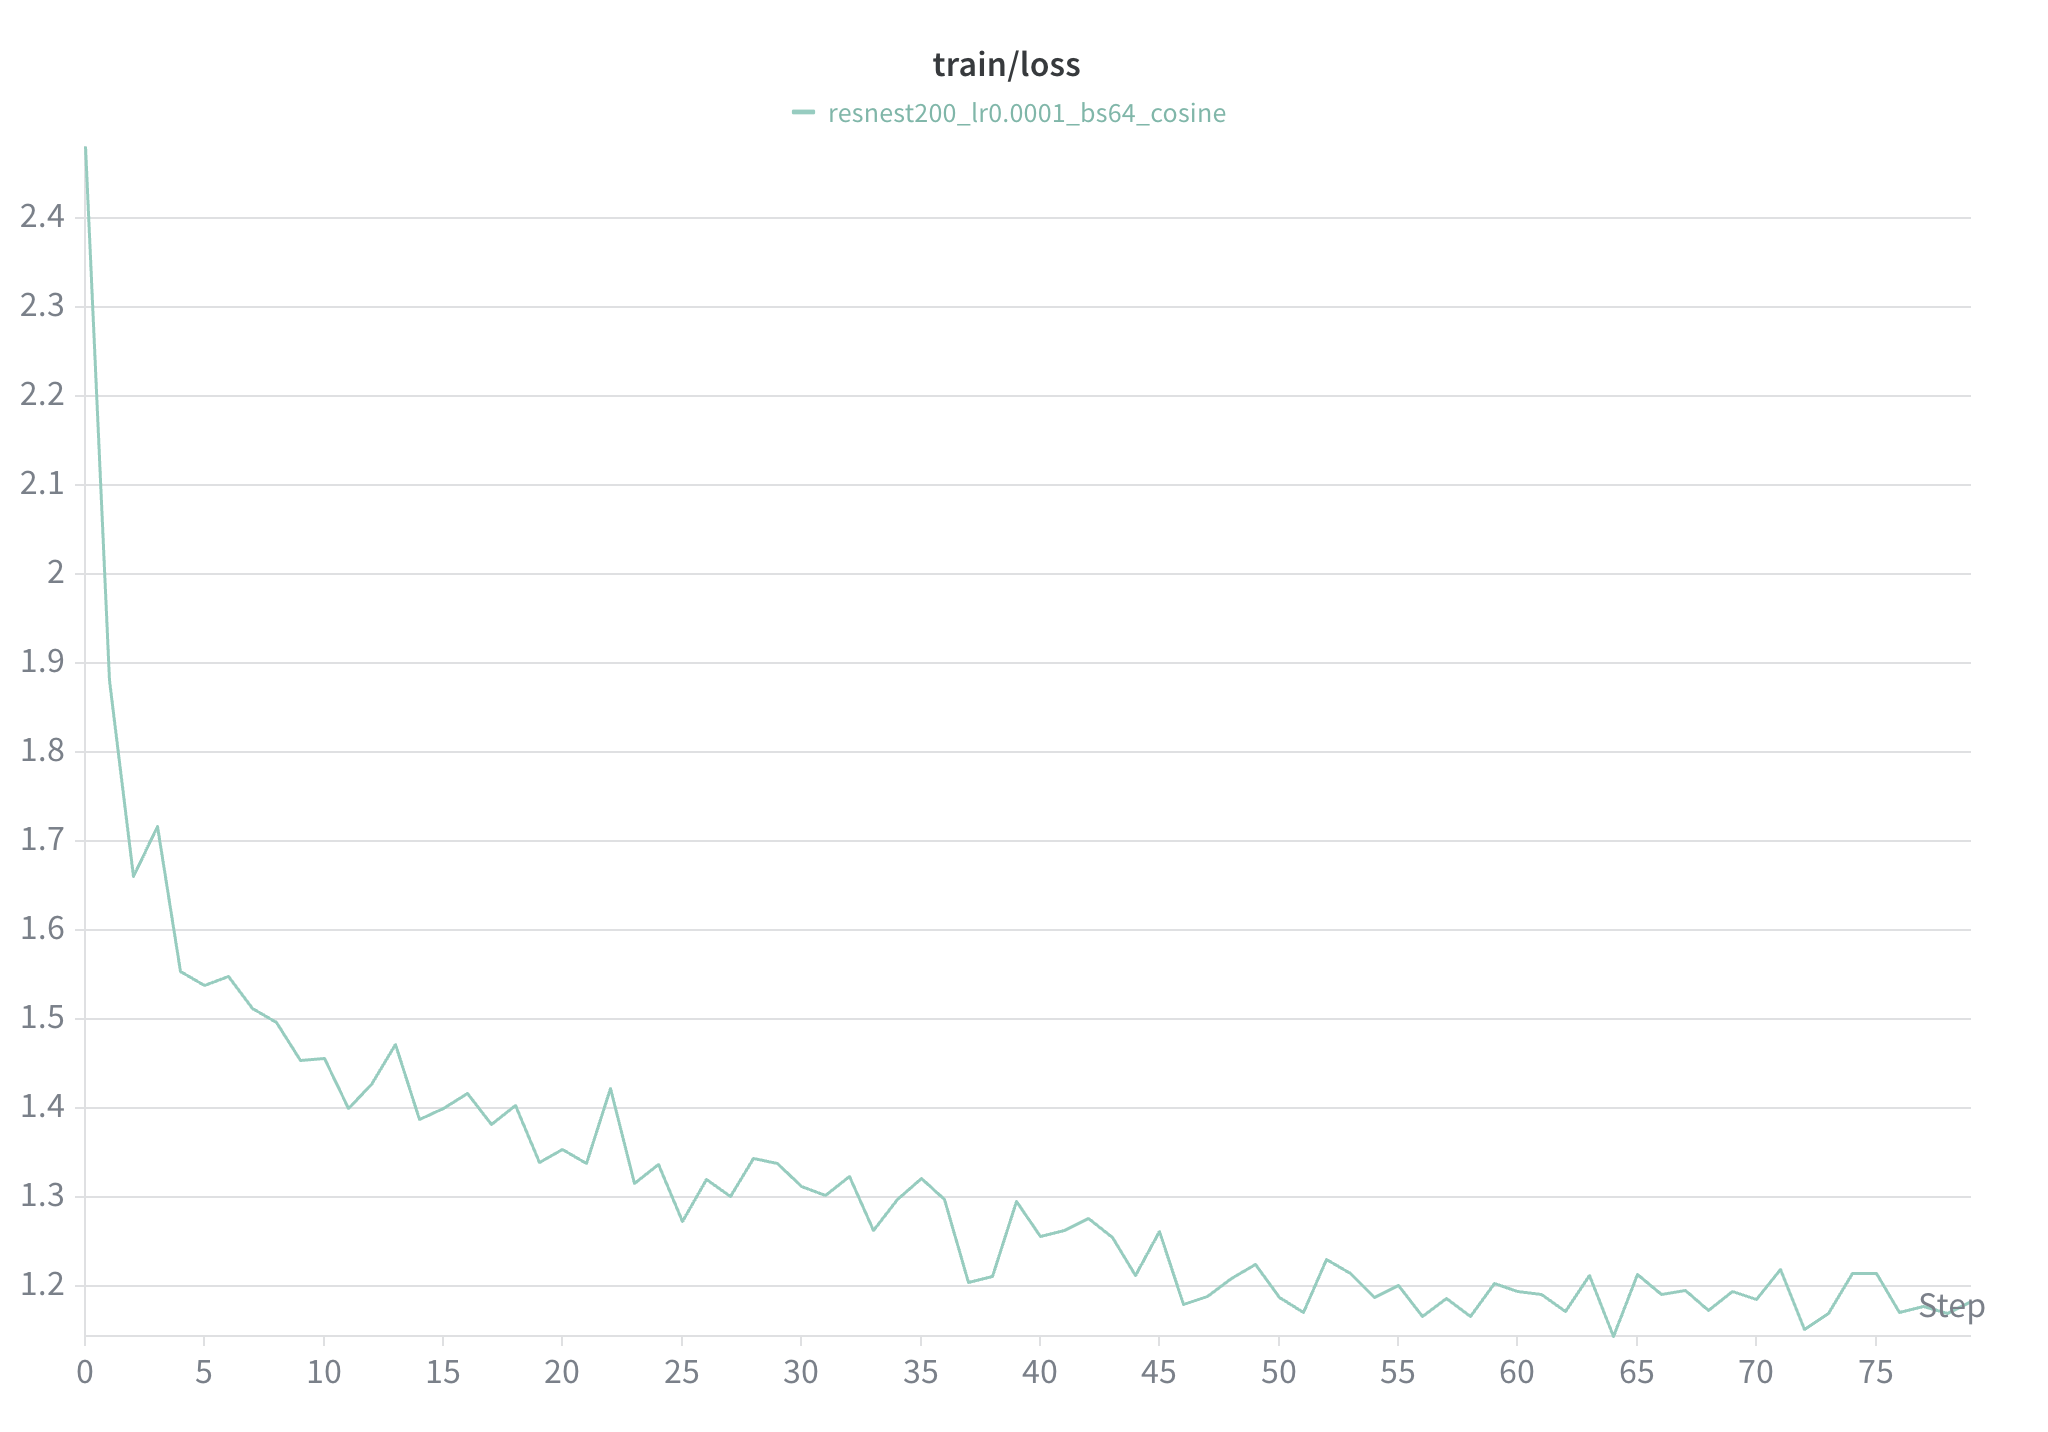
\includegraphics[width=\linewidth]{assets/train_loss.png}
		\caption{Training loss}
		\label{fig:train_loss}
	\end{subfigure}
	\hfill
	\begin{subfigure}{0.48\linewidth}
		\centering
		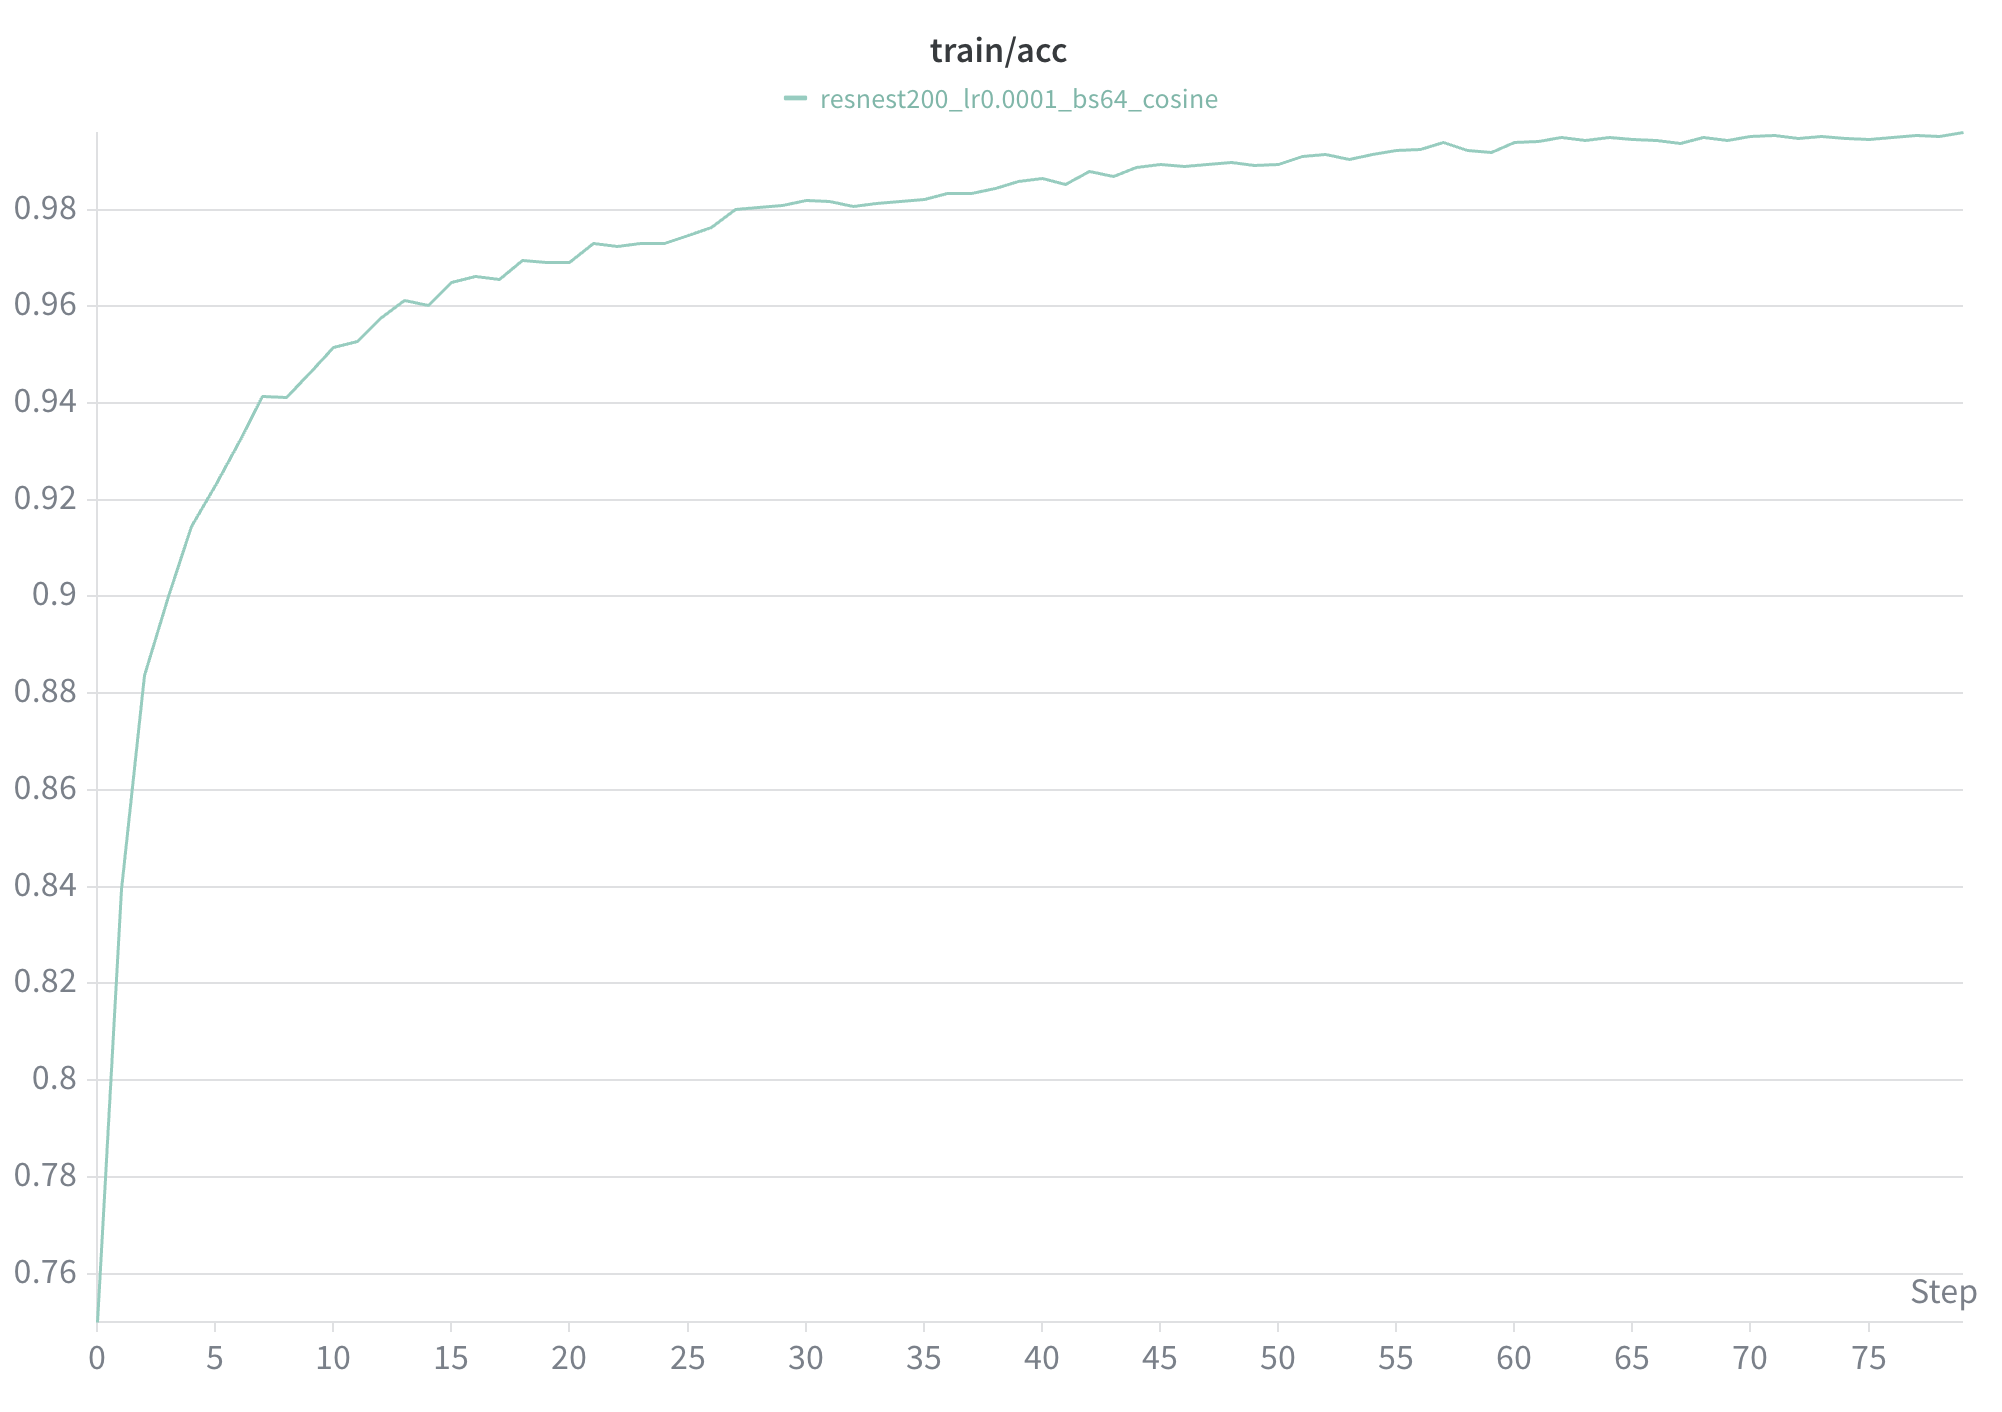
\includegraphics[width=\linewidth]{assets/train_acc.png}
		\caption{Training accuracy}
		\label{fig:train_acc}
	\end{subfigure}

	\vspace{0.3cm}

	\begin{subfigure}{0.48\linewidth}
		\centering
		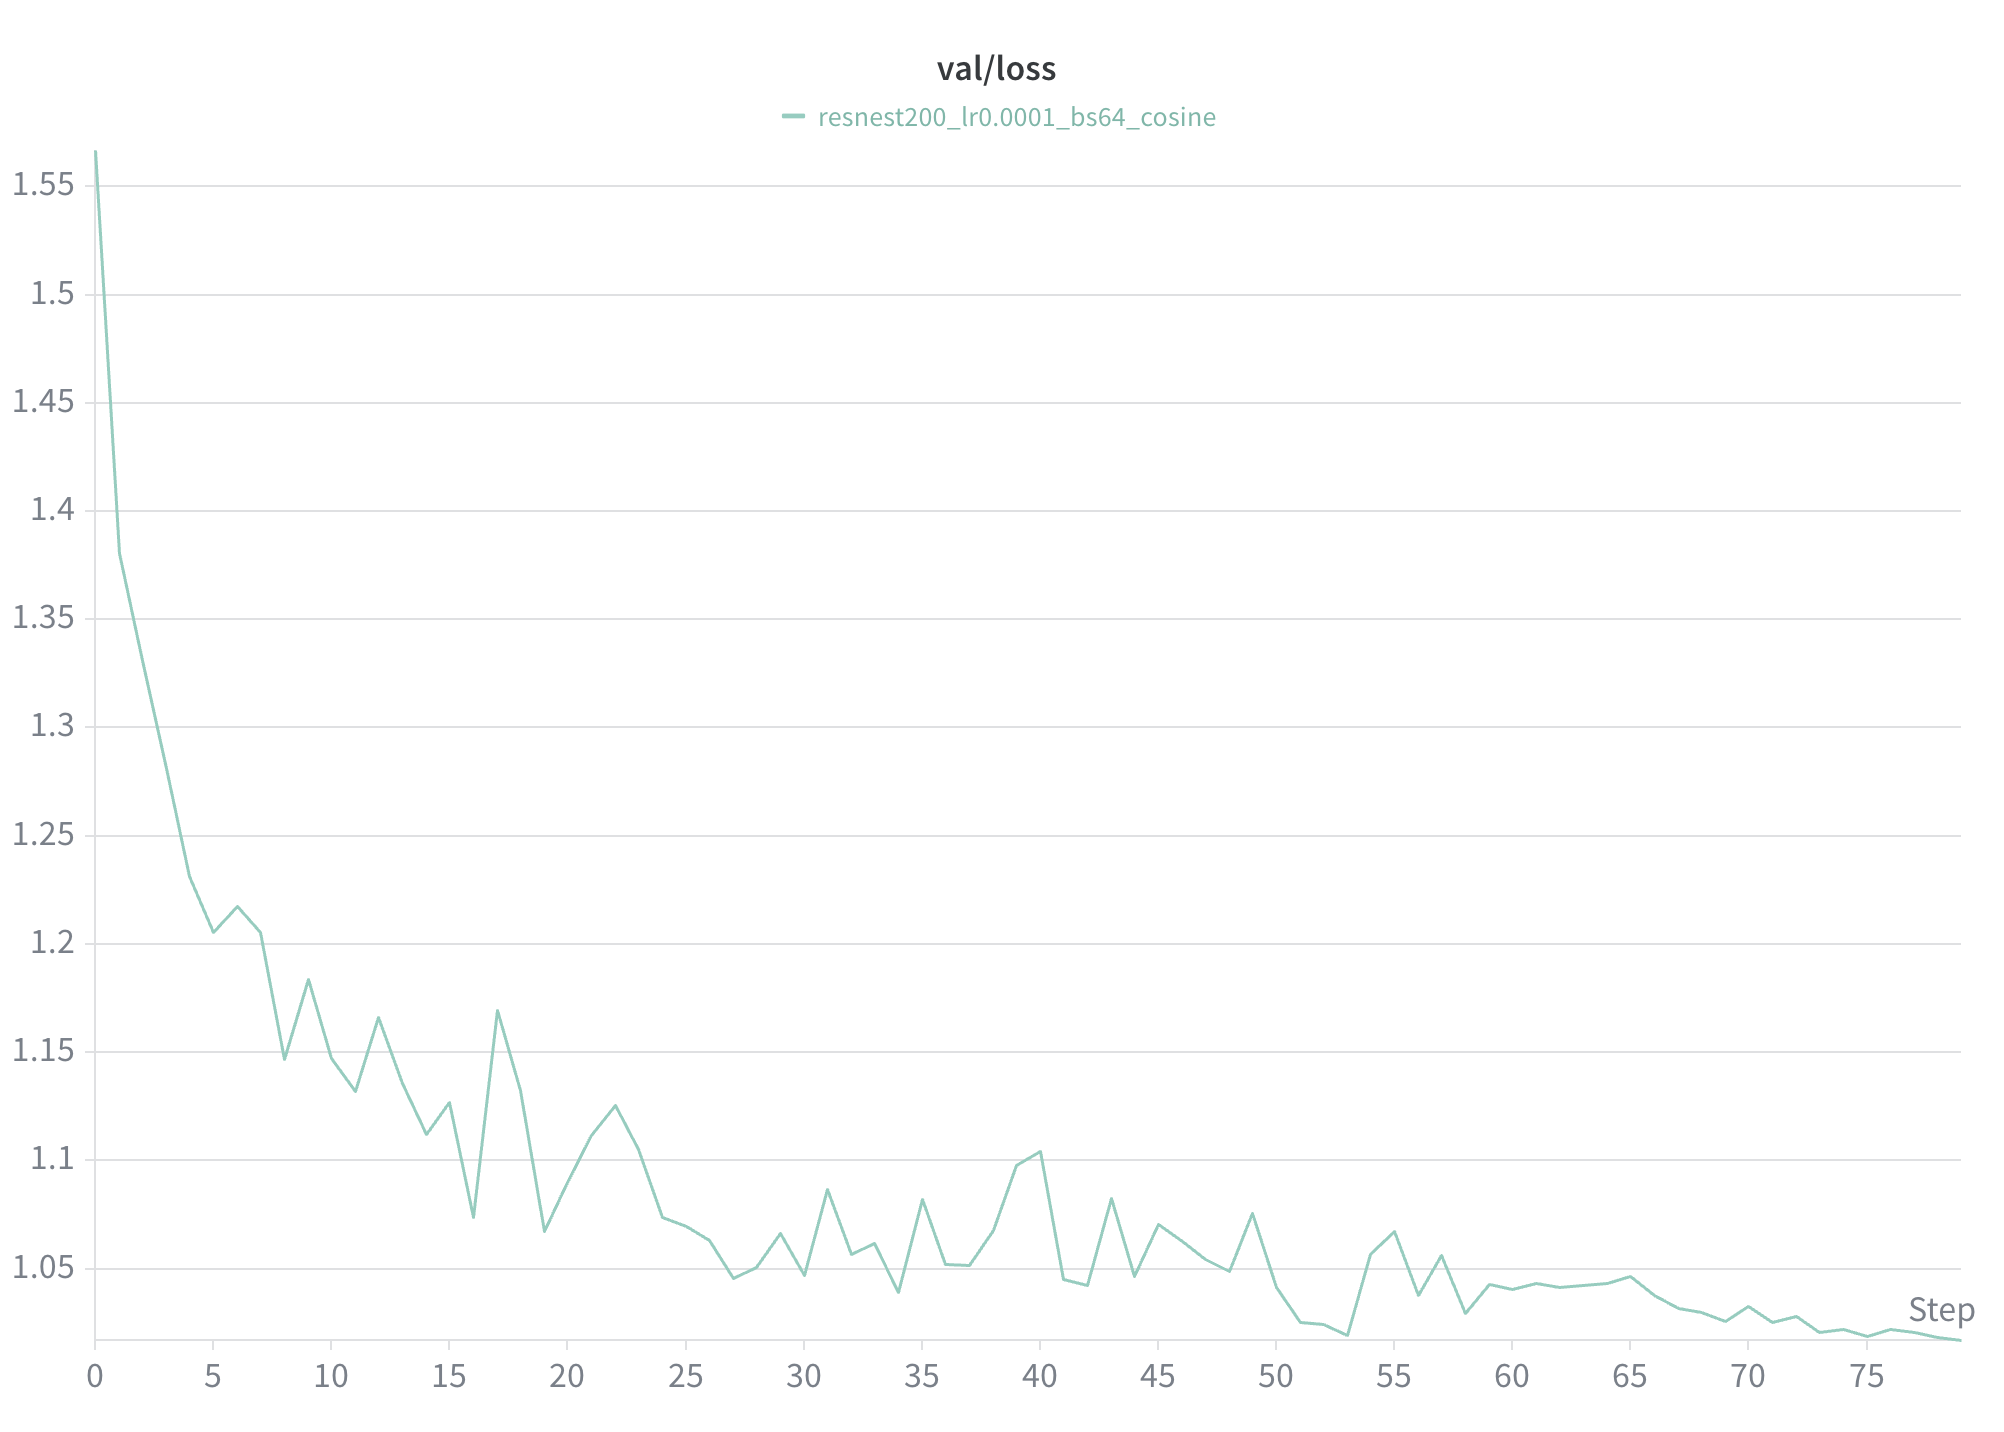
\includegraphics[width=\linewidth]{assets/val_loss.png}
		\caption{Validation loss}
		\label{fig:val_loss}
	\end{subfigure}
	\hfill
	\begin{subfigure}{0.48\linewidth}
		\centering
		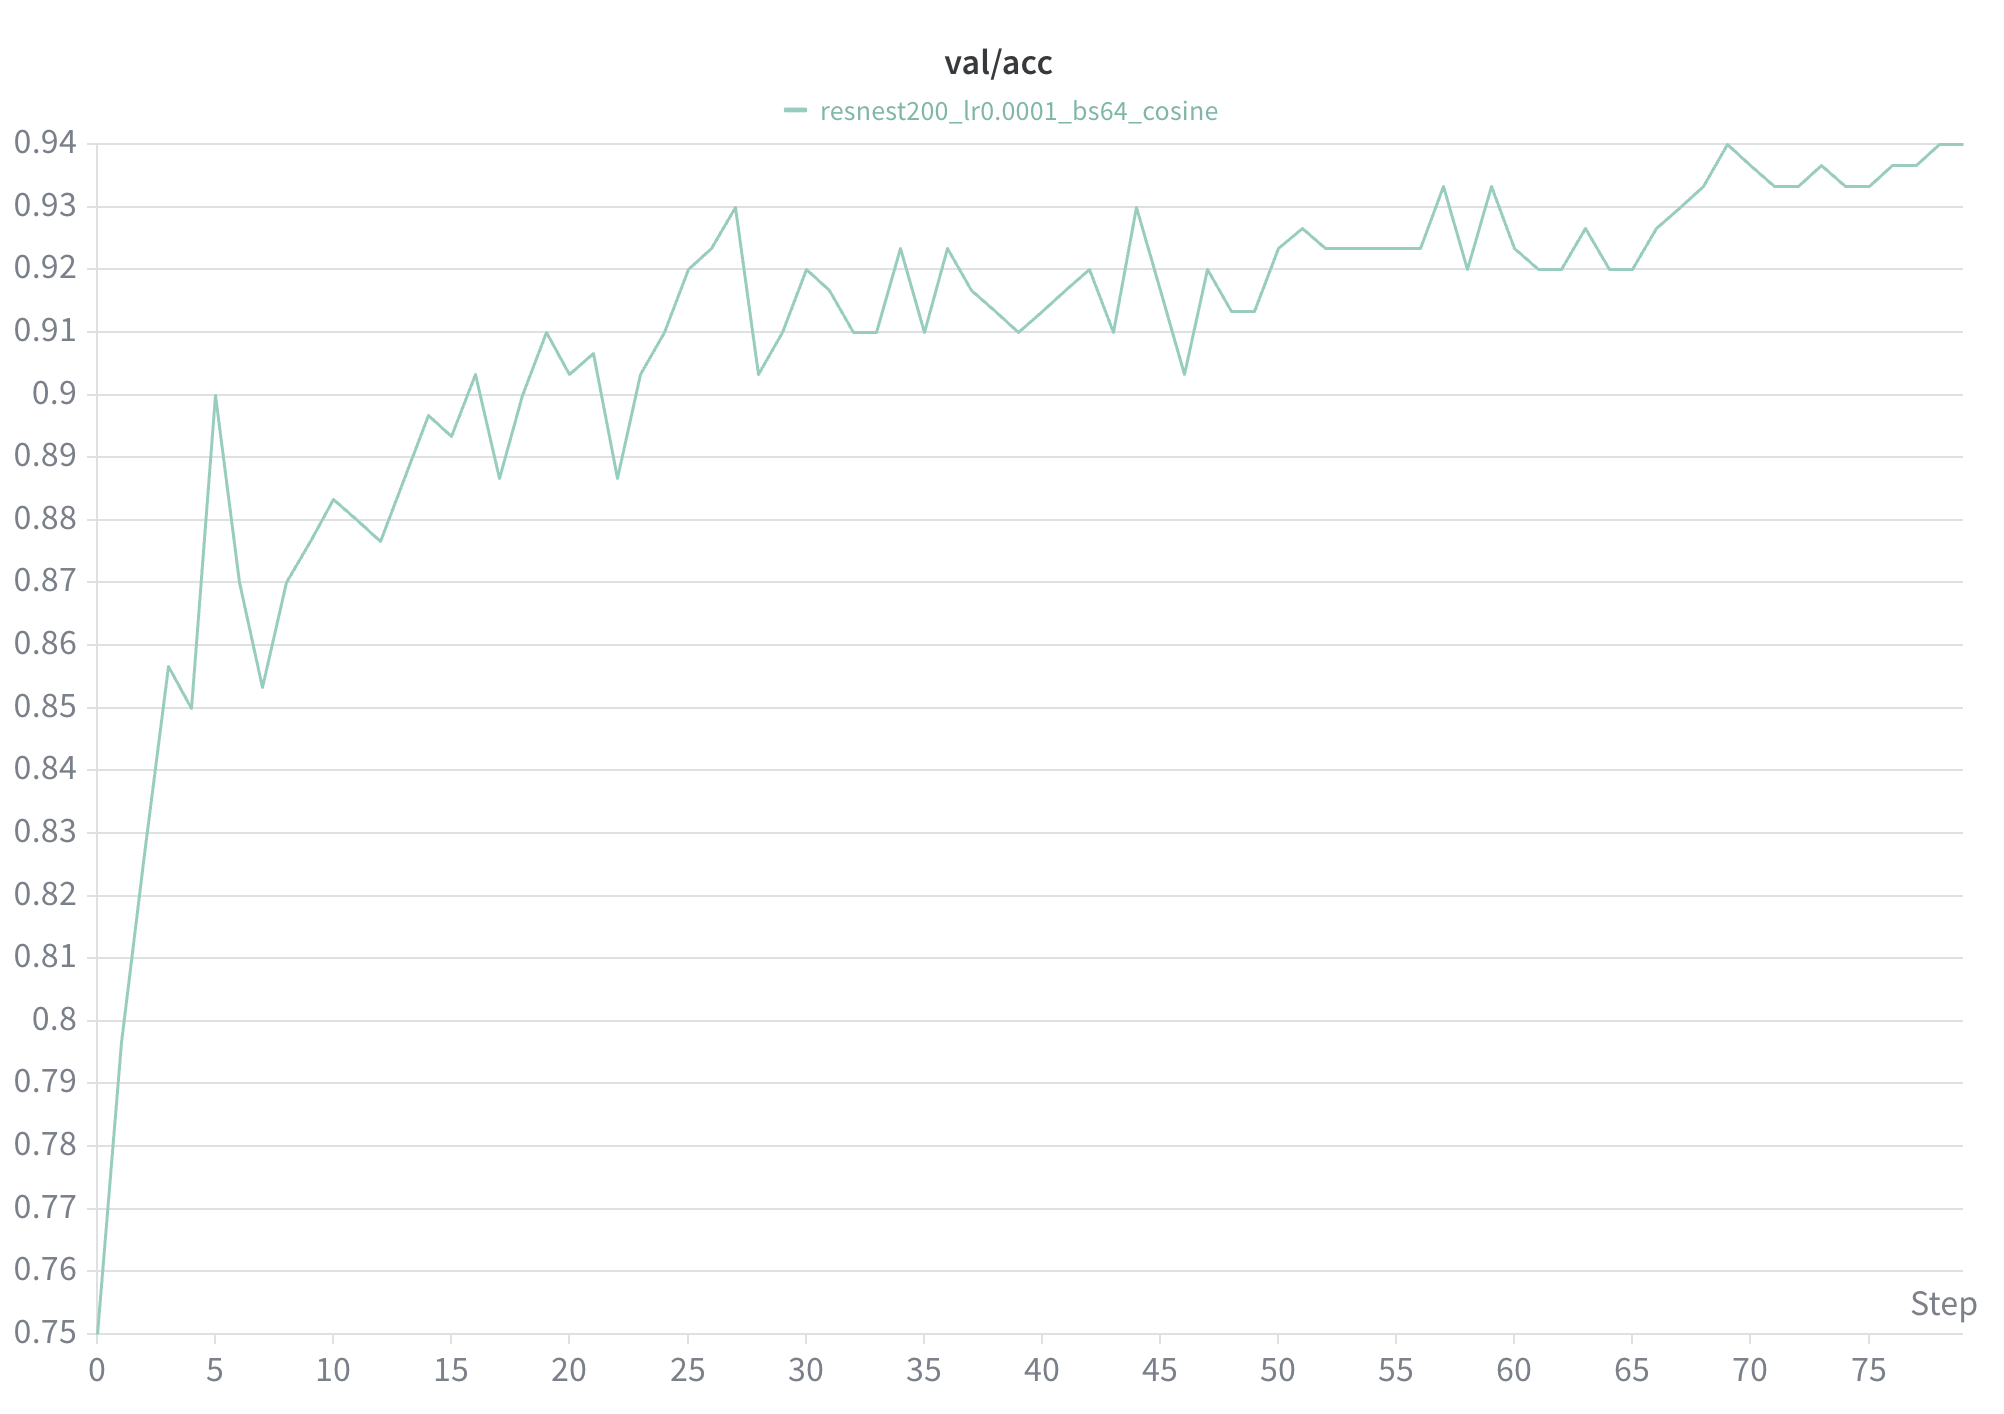
\includegraphics[width=\linewidth]{assets/val_acc.png}
		\caption{Validation accuracy}
		\label{fig:val_acc}
	\end{subfigure}
	\caption{Training and validation curves over 80 epochs for ResNeSt-200 with cosine annealing scheduler, no dropout, and image size $224 \times 224$.}
	\label{fig:train_curves}
\end{figure}

\subsection{Competition Performance}
\label{sec:competition}

With TTA enabled during inference, our best model achieves a test accuracy of \textbf{0.96} on the CodaBench competition leaderboard, as shown in \cref{fig:competition}. The notable gap between the validation accuracy (94\%) and test accuracy (96\%) suggests that TTA provides a meaningful boost by aggregating predictions across multiple augmented views, effectively reducing variance in the final predictions.

\begin{figure}[t]
	\centering
	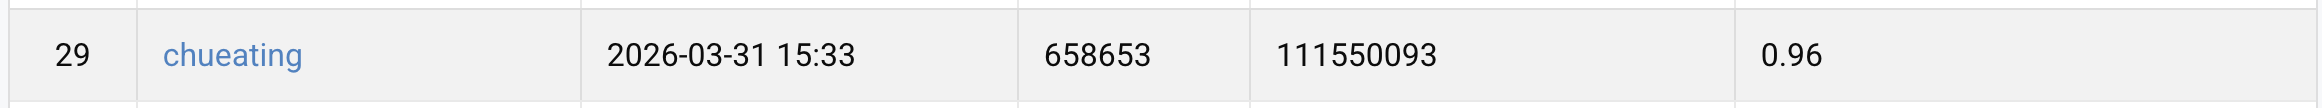
\includegraphics[width=\linewidth]{assets/competition.png}
	\caption{CodaBench leaderboard screenshot showing our test accuracy of 0.96.}
	\label{fig:competition}
\end{figure}

%------------------------------------------------------------------------
\section{Experiments}
\label{sec:experiments}

\subsection{Effect of Dropout Rate}
\label{sec:exp_dropout}

Zhang and Bottou~\cite{zhang2024finetune_large_dropout} recently demonstrated that applying very large dropout rates (\eg, 90\%) on the penultimate layer during fine-tuning can improve out-of-distribution generalization, sometimes exceeding deep ensembles and model soups. Motivated by this finding, we compare dropout rates of 0.0 and 0.9 applied before the final classification layer, with all other settings held constant (ResNeSt-200, cosine scheduler, $\text{lr} = 10^{-4}$, image size $224 \times 224$).

\begin{table}[t]
	\centering
	\begin{tabular}{lcc}
		\toprule
		\textbf{Dropout Rate} & \textbf{Best Val Acc (\%)} & \textbf{Best Epoch} \\
		\midrule
		0.0                   & \textbf{93.00}             & 71                  \\
		0.9                   & 92.33                      & 45                  \\
		\bottomrule
	\end{tabular}
	\caption{Validation accuracy comparison between dropout rates of 0.0 and 0.9. Both models use the cosine annealing scheduler with identical hyperparameters.}
	\label{tab:dropout}
\end{table}

As shown in \cref{tab:dropout} and \cref{fig:dropout}, the standard configuration without dropout achieves a slightly higher validation accuracy of 93.00\% compared to 92.33\% with dropout 0.9. We hypothesize that the extremely aggressive dropout rate, while beneficial for out-of-distribution scenarios as reported by Zhang and Bottou~\cite{zhang2024finetune_large_dropout}, may be overly restrictive for our in-distribution evaluation setting where the validation and test sets share similar characteristics with the training data. Additionally, the heavy augmentation pipeline (TrivialAugment, CutMix, MixUp, Random Erasing, and label smoothing) already provides substantial regularization, potentially making the additional dropout redundant or even harmful to training convergence.

\begin{figure}[t]
	\centering
	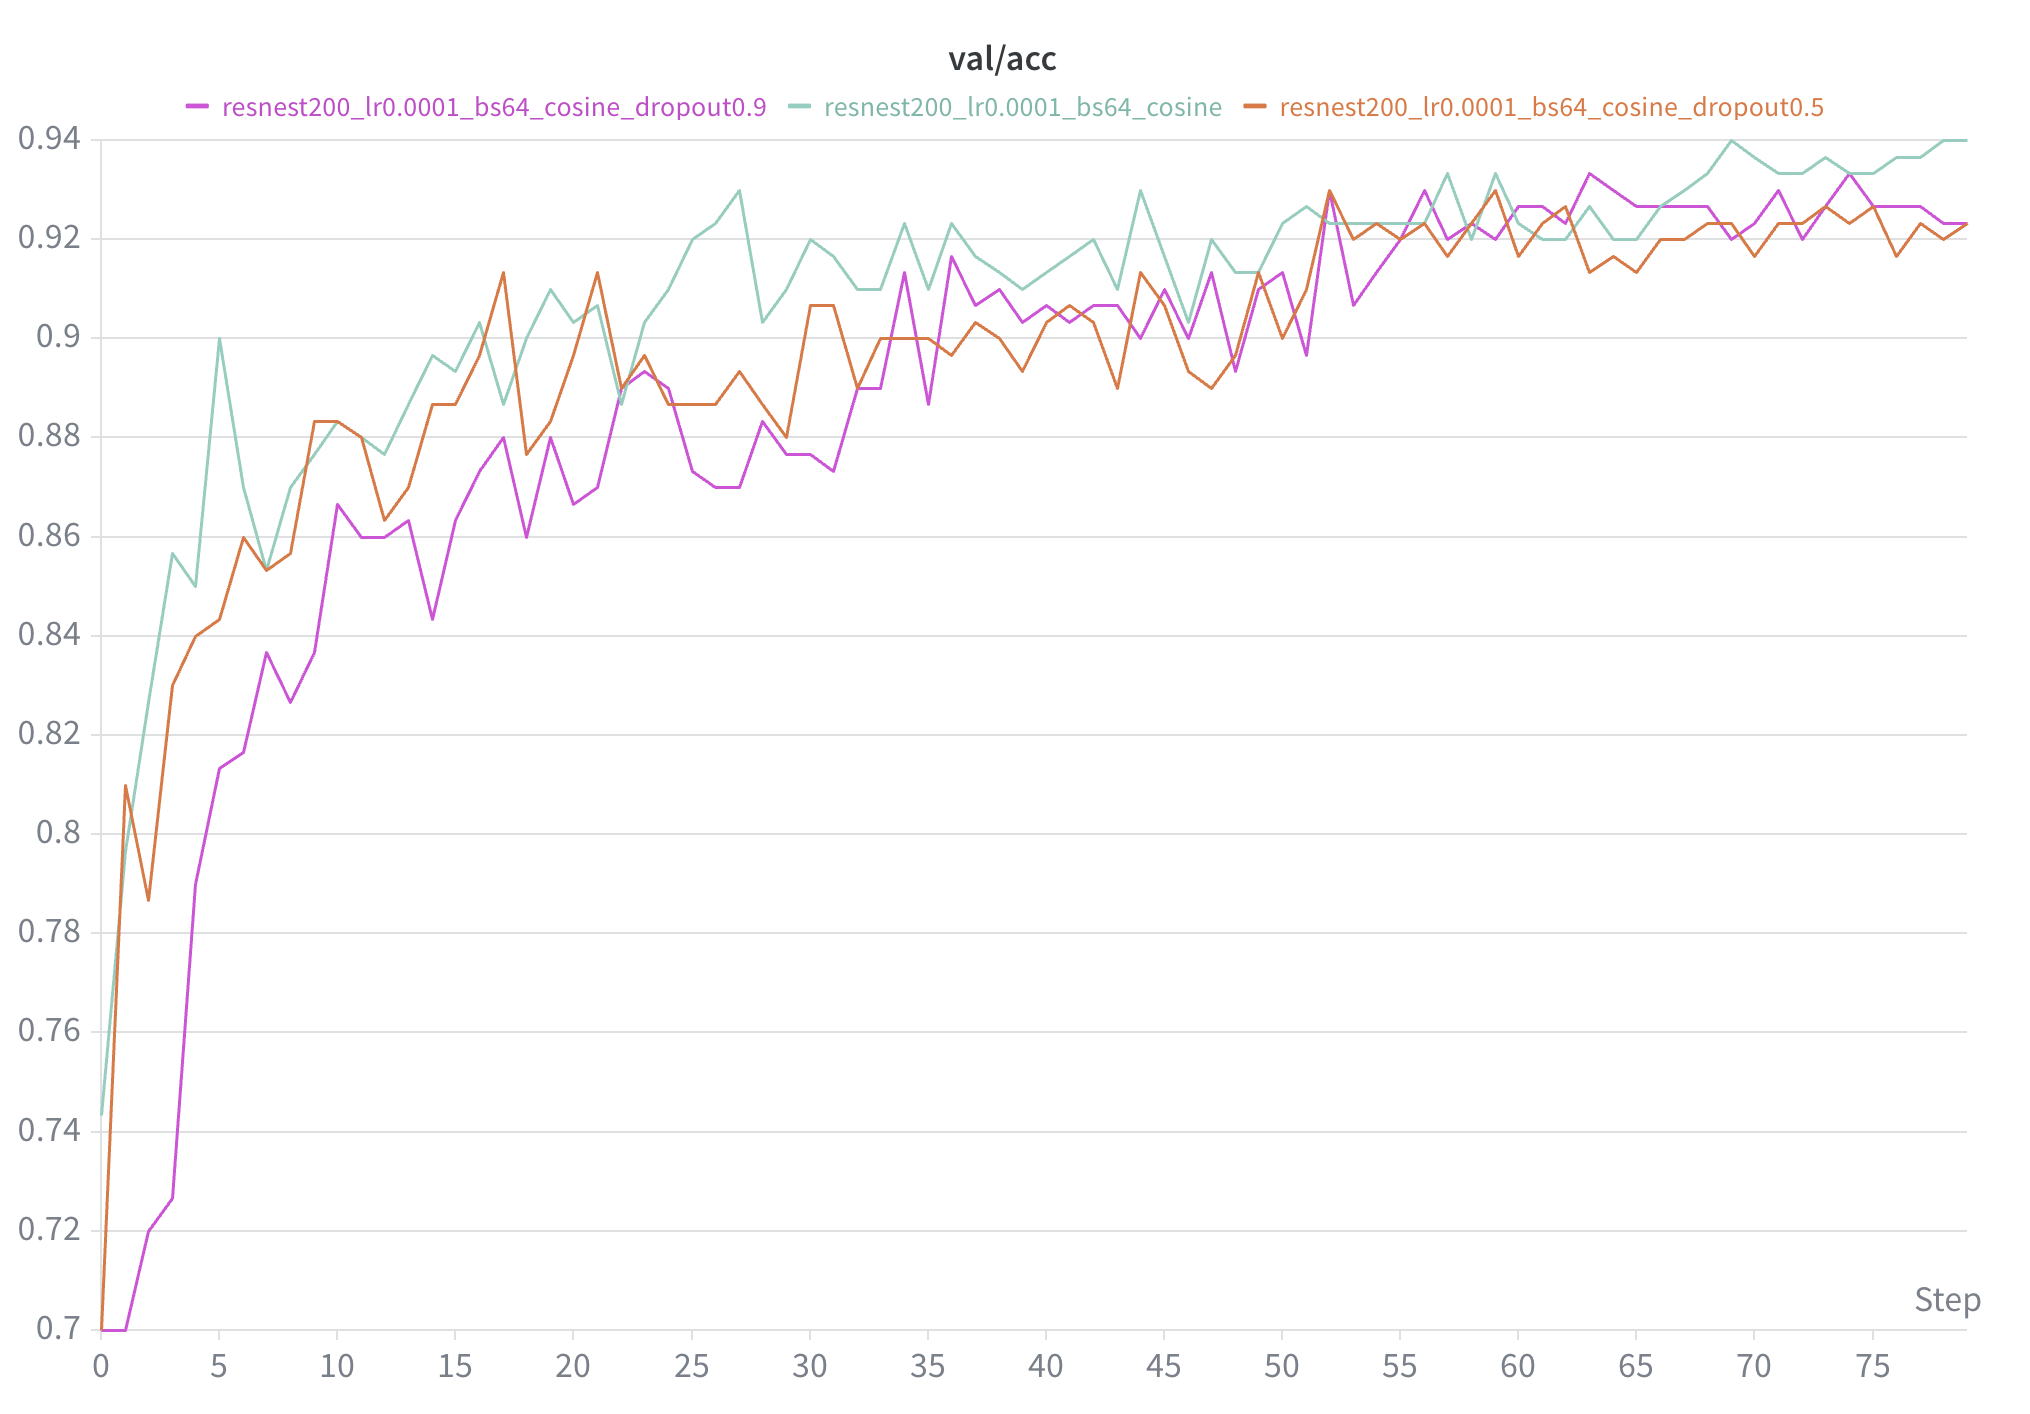
\includegraphics[width=\linewidth]{assets/exp/dropout.png}
	\caption{Validation accuracy curves comparing dropout rates of 0.0 and 0.9 over training epochs. The model without dropout achieves higher peak accuracy and more stable convergence.}
	\label{fig:dropout}
\end{figure}

\subsection{Effect of Learning Rate Scheduler}
\label{sec:exp_scheduler}

We compare four learning rate scheduling strategies, all using ResNeSt-200 with dropout 0.0, $\text{lr} = 10^{-4}$, and image size $224 \times 224$:

\begin{itemize}
	\item \textbf{Cosine Annealing}~\cite{loshchilov2017sgdr}: Smoothly decays the learning rate following a cosine curve from $\text{lr}$ to $\eta_{\min} = 10^{-6}$ over $T_{\max} = 80$ epochs.
	\item \textbf{OneCycleLR}~\cite{smith2019onecycle}: Ramps the learning rate up to the maximum during the first 10\% of training, then anneals it to near zero.
	\item \textbf{ReduceLROnPlateau}: Reduces the learning rate by a factor of 0.1 when the validation loss plateaus for 5 consecutive epochs.
	\item \textbf{Cosine Annealing with Warm Restarts}~\cite{loshchilov2017sgdr}: Periodically resets the learning rate with $T_0 = 10$ and $T_{\text{mult}} = 2$, creating increasingly longer annealing cycles.
\end{itemize}

\begin{table}[t]
	\centering
	\begin{tabular}{lcc}
		\toprule
		\textbf{Scheduler} & \textbf{Best Val Acc (\%)} & \textbf{Best Epoch} \\
		\midrule
		Cosine Annealing   & \textbf{94.00}             & 69                  \\
		OneCycleLR         & 93.67                      & 76                  \\
		Plateau            & 93.33                      & 45                  \\
		Warm Restarts      & 93.00                      & 28                  \\
		\bottomrule
	\end{tabular}
	\caption{Validation accuracy comparison across learning rate schedulers. All models use ResNeSt-200, dropout 0.0, and identical hyperparameters. The Cosine Annealing result corresponds to \texttt{checkpoints/best.pth}.}
	\label{tab:scheduler}
\end{table}

As shown in \cref{tab:scheduler} and \cref{fig:scheduler}, Cosine Annealing achieves the highest validation accuracy of 94.00\%, followed closely by OneCycleLR at 93.67\%. ReduceLROnPlateau and Warm Restarts trail slightly at 93.33\% and 93.00\%, respectively.

Cosine Annealing benefits from a smooth, monotonic decay that allows the model to gradually settle into a sharp minimum during the later stages of training. OneCycleLR performs comparably, as its warmup phase helps escape poor local minima early on. ReduceLROnPlateau, while adaptive, can be sensitive to the patience hyperparameter and may reduce the learning rate prematurely or too late. Warm Restarts achieves its best accuracy early (epoch 28) but the periodic learning rate resets can destabilize learned features, preventing consistent improvement over longer training.

\begin{figure}[t]
	\centering
	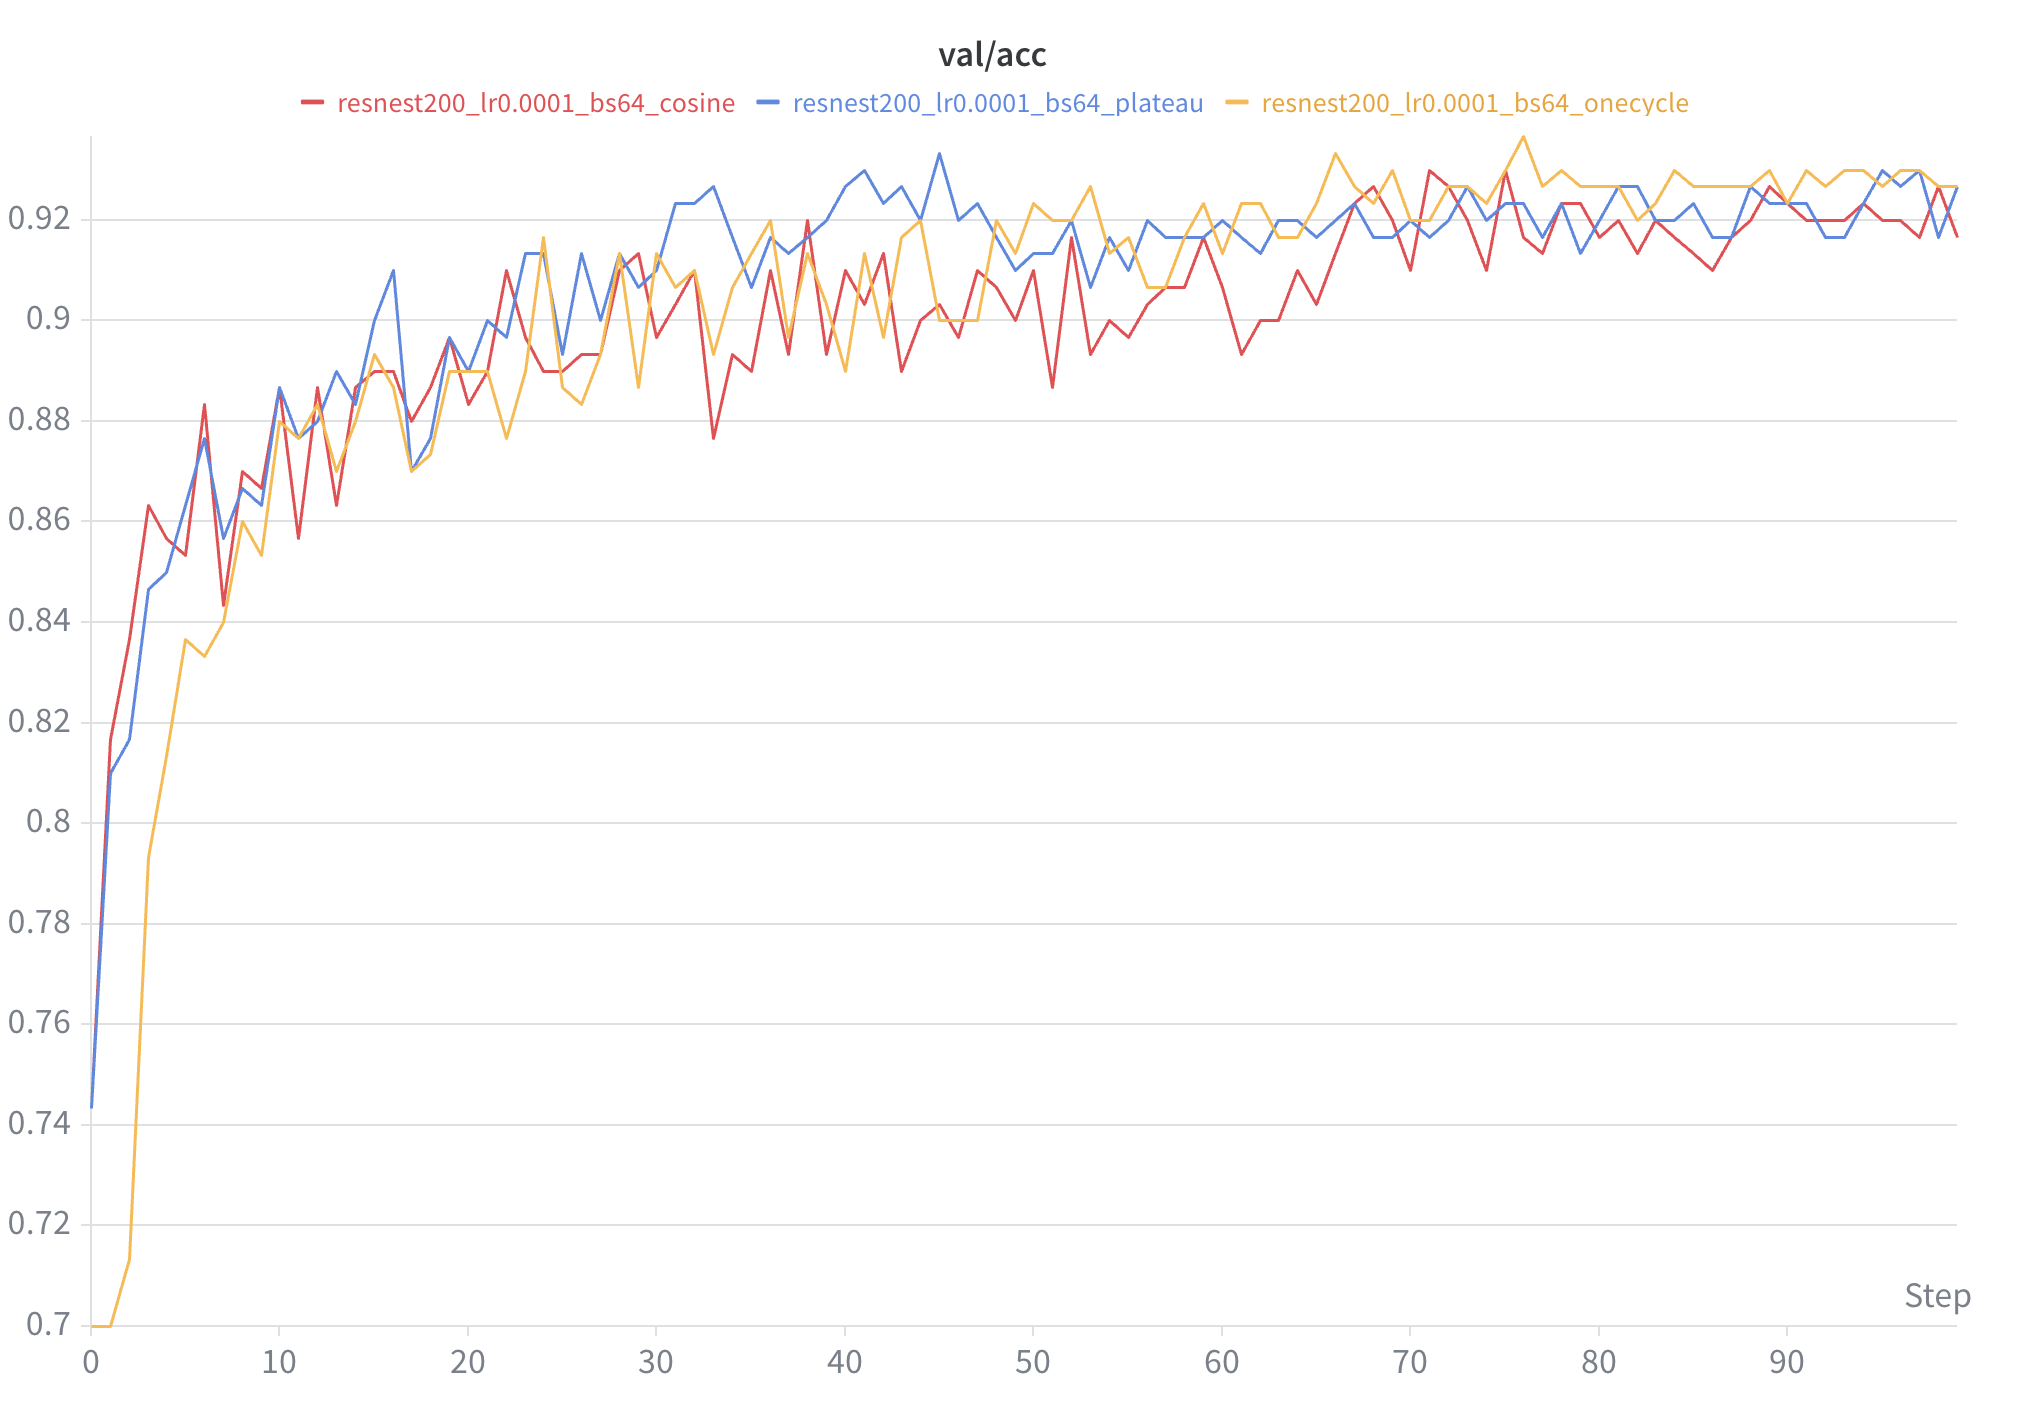
\includegraphics[width=\linewidth]{assets/exp/scheduler.png}
	\caption{Validation accuracy curves for different learning rate schedulers over training epochs.}
	\label{fig:scheduler}
\end{figure}

%------------------------------------------------------------------------

{\small
\bibliographystyle{ieee_fullname}
\bibliography{egbib}
}

\end{document}
